\documentclass[a4paper,12pt]{article} % тип документа
\usepackage[margin=1in]{geometry} % Поля

%  Русский язык
\usepackage[warn]{mathtext}
\usepackage[T2A]{fontenc}			% кодировка
\usepackage[utf8]{inputenc}			% кодировка исходного текста
\usepackage[english,russian]{babel}	% локализация и переносы
% Математика
\usepackage{amsmath,amsfonts,amssymb,amsthm,mathtools} 
\usepackage{wasysym}
%%%
\usepackage{graphicx}

\usepackage{tabularx}

\usepackage{gensymb} % знак градуса
\usepackage{enumitem} % изменить список enumerate
\usepackage{placeins} % \FloatBarrier

\renewcommand{\thesection}{\Roman{section}} 
\renewcommand{\thesubsection}{\roman{subsection}}


\begin{document}

\newcolumntype{Y}{>{\centering\arraybackslash}X} %new tabularx


%титул
\hrule 	
\medskip
\begin{raggedright}
{\large \textbf{Отчёт по работе 5.1.3}}
\\
\medskip
{\Large Изучение рассеяния медленных электронов на атомах (эффект Рамзауэера)} 
\\
\medskip
{\large Бичина Марина, Карташов Констанин Б04-005}
\medskip
\hrule
\medskip
\end{raggedright}


\section{Анотация}

\paragraph{Цель работы:} 
Исследовать энергетическую зависимость вероятности рассеяния электронов атомам ксенона, определение энергии электроном, при которых наблюдается <<просветление>> ксенона, и оценить размер его внешней электронной оболочки.

\paragraph{Оборудование:}
\begin{itemize}
\renewcommand{\labelitemi}{$\triangleright$}
\itemsep0em
\item Тиратрон
\item Источник переменного и постоянного напряжения
\item Электронный осциллограф
\item Вольтметры
\end{itemize}


\medskip\hrule\medskip

\section{Теоретическая часть}

\paragraph{} Из условия первого интерференционного максимума ($\Delta = 2l = \lambda'$) можно рассчитать размер потенциальной ямы $l$, как:

\begin{equation}\label{e:max}
l = \frac{1}{2} \frac{h}{\sqrt{2m(E_{\max} + U_0)}},
\end{equation}

\noindent из условия первого интерференционного минимума ($\Delta = 2l = 3/2 \lambda'$) можно рассчитать $l$ как:

\begin{equation}\label{e:min}
l = \frac{3}{4} \frac{h}{\sqrt{2m(E_{\min} + U_0)}}.
\end{equation}

Совмещая \eqref{e:max} и \eqref{e:min} можно рассчитать $l$ и $U_0$ по формулам:

\begin{equation}\label{e:l}
l = \frac{h\sqrt{5}}{\sqrt{32m(E_{\min} - E_{\max})}},
\end{equation}

\begin{equation}\label{e:u_0}
U_0 = \frac{4}{5} E_{\min} - \frac{9}{5} E_{\max}.
\end{equation}

\paragraph{} По измеренной вольт-амперной характеристике можно определить зависимость вероятности рассеяние электрона от его энергии из соотношения:

\begin{equation}\label{e:prob}
w(V) = - \frac{1}{C} \ln{\frac{I_\text{анод}(V)}{I_\text{катод}}}
\end{equation}

\medskip\hrule\medskip

\FloatBarrier
\section{Экспериментальная часть}

\subsection{Вольт-амперная характеристика тиратрона в динамическом режиме}\label{ss:dynamic}

\paragraph{} Включим установку в динамическом режиме, выставим установим напряжение накала $V_1 = 3.05$ В и получим на экране осциллографа изображение кривой вольт-амперной характеристики (рис. \ref{fig:scope} (а)). Зная, что одно деление по оси $X$ осциллографа соответствует 2 В, найдём напряжения первого максимума и минимума, и  напряжение пробоя: 

$U_{\max} = 1.35$ дел $= 2.7$ В, оценим погрешность $\sigma_{U_{\max}} \approx 0.05$ дел $= 0.1$ В, $U_{\min} = 3.15$ дел = $ 6.3$ В, оценим погрешность $\sigma_{U_{\min}} \approx 0.35$ дел $= 0.7$ В, $U_\text{проб} = 6$ дел $= 12$ В.

\paragraph{} Изменим напряжение на накала до $V_2 = 2.75$ В. Изображение на экране осциллографа изменилось (рис. \ref{fig:scope} (б)). Также найдём напряжения первого максимума и минимума, и  напряжение пробоя: 

$U_{\max} = 1.35$ дел $= 2.7$ В, оценим погрешность $\sigma_{U_{\max}} \approx 0.05$ дел $= 0.1$ В, $U_{\min} = 2.75$ дел = $ 5.5$ В, оценим погрешность $\sigma_{U_{\min}} \approx 0.35$ дел $= 0.7$ В, $U_\text{проб} = 6$ дел $= 12$ В.

Измеренные данные занесём в таблицу \ref{tab:dynamic}.

\paragraph{} По измеренным данным оценим размер электронной оболочки атома инертного газа, заполняющего лампу, приняв $U_0 = 2.5$ В по формулам \eqref{e:max} и \eqref{e:min}, получим: $l_1 = 2.7 \pm 0.1 $ Å, $l_2 = 3.1 \pm 0.3 $ Å, $l_3 = 2.7 \pm 0.1 $ Å, $l_4 = 3.3 \pm 0.4 $ Å для $V_{\max}$ и $V_{\min}$ при $V_1$ и $V_2$ соответственно. Среднее и среднеквадратичное отклонение: $\bar{l} = 2.95$ Å, $\sigma_l = 0.26$ Å.

Найдём $l$ по формуле \eqref{e:l}, получим: $l_1 = 3.6 \pm 0.4$ Å, $l_2 = 4.1 \pm 0.5$ Å для $V_1$ и $V_2$ соответственно. Среднее и среднеквадратичное отклонение: $\bar{l} = 3.85$ Å, $\sigma_l = 0.25$ Å. 

Найдём соответствующие значения размера потенциальной ямы $U_0$ по формуле \eqref{e:u_0}: $U_{0,1} = 0.2 \pm 0.6$ В, $U_{0,1} = -0.5 \pm 0.6$ -- эти значения явно не соответствуют действительности, так как их модуль меньше погрешности, и отрицательное значение не должно быть возможным. Такие ошибки могли возникнуть из-за некачественного изображения полученного на осциллографе. Занесём вычислинные значения в таблицу \ref{tab:dynamic_res}.

\paragraph{} Оценим потенциал ионизации инертного газа. Напряжение пробоя получилось $V_\text{проб} \approx 12$ В, что соответствует ионизационному потенциалу ксенона -- $12.1$ эВ. Из этого можно заключить, что тиратрон заполнен ксеноном.


\begin{table}[]
\centering
\begin{tabular}{|c|c|c|c|c|c|}
\hline
измерение & $V_\text{нак}$, В & $V_{\max}$, В & $\sigma_{V_{\max}}$, В & $V_{\min}$, В & $\sigma_{V_{\min}}$, В \\ \hline
1         & 3.05              & 2.7           & 0.1                    & 6.3           & 0.7                    \\ \hline
2         & 2.75              & 2.7           & 0.1                    & 5.5           & 0.7                    \\ \hline
\end{tabular}
\caption{Значения измеренные динамическим методом}
\label{tab:dynamic}
\end{table}

\begin{table}[]
\centering
\begin{tabular}{|c|c|c|c|c|c|c|c|c|}
\hline
формула, $V_i$ & \eqref{e:max}, 1 & \eqref{e:min}, 1 & \eqref{e:max}, 2 & \eqref{e:min}, 2 & сред. & \eqref{e:l}, 1 & \eqref{e:l}, 2 & сред. \\ \hline
$l$, Å         & 2.7  & 3.1  & 2.7  & 3.3  & 2.95 & 3.6                       & 4.1                       & 3.85                      \\ \hline
$\sigma_l$, Å  & 0.1  & 0.3  & 0.1  & 0.4  & 0.26 & 0.4                       & 0.5                       & 0.25                      \\ \hline
\end{tabular}
\caption{Значения найденные динамическим методом}
\label{tab:dynamic_res}
\end{table}

\begin{figure}
\centering
\begin{minipage}{0.49\textwidth}
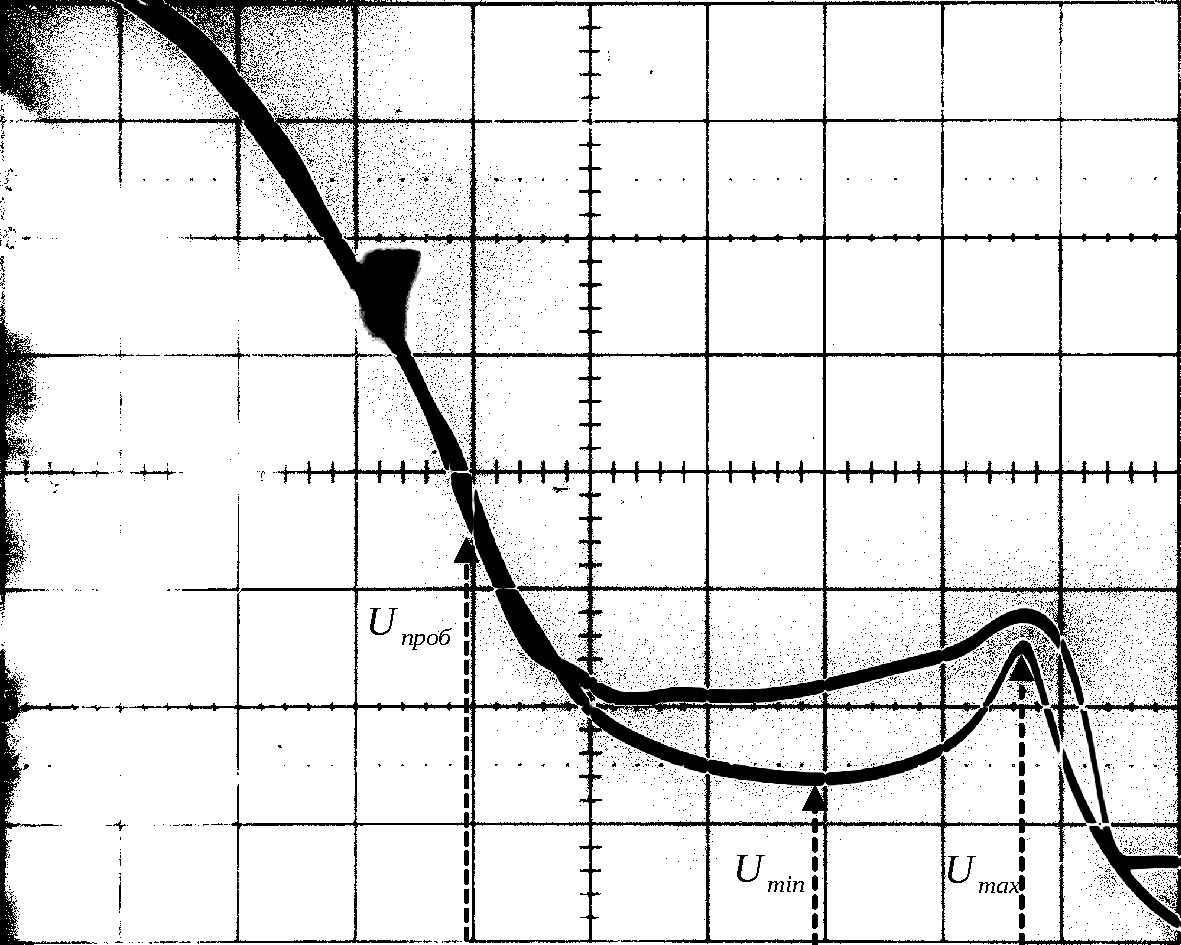
\includegraphics[width=\textwidth]{scope_hv.pdf}
\center{а)}
\end{minipage}
\begin{minipage}{0.49\textwidth}
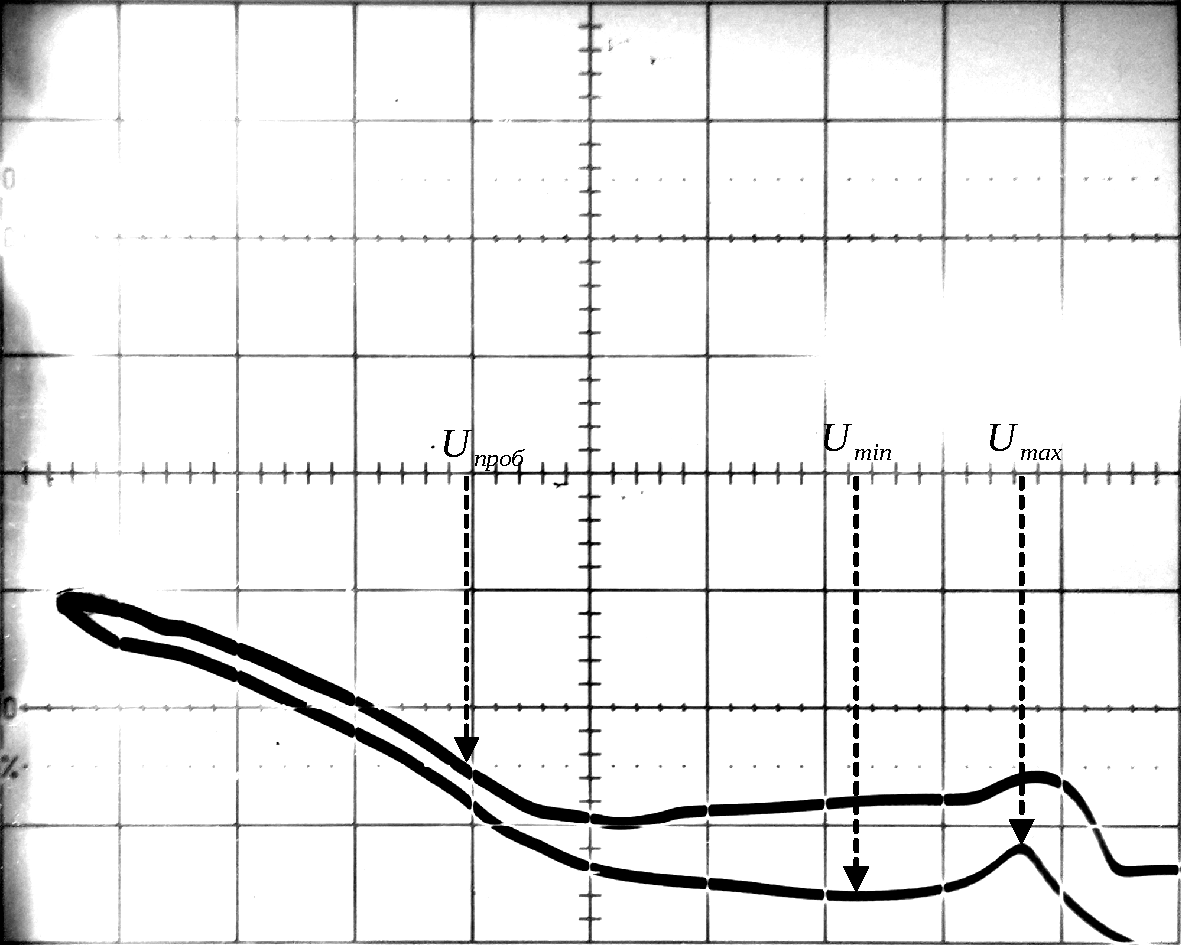
\includegraphics[width=\textwidth]{scope_lv.pdf}
\center{б)}
\end{minipage}
\caption{Кривые на экране осциллографа при а) $V_\text{накал} = V_1$ б) $V_\text{накал} = V_2$}
\label{fig:scope}
\end{figure}
\medskip\hrule\medskip

\subsection{Вольт-амперная характеристика тиратрона в статическом режиме}

\paragraph{} Переведём установку в статический режим. При мощи двух вольтметров показывающих напряжение и ток (в относительных единицах) построим вольт-амперную характеристику при напряжениях накала близких к $V_1$ и $V_2$ из п.п. \ref{ss:dynamic} (рис. \ref{fig:static}).

\paragraph{} Полученные напряжения $V_{\max, 1} = 2.36$ В, $V_{\max, 2} = 2.39$ В, $V_{\min, 1} = 7.00$ В, $V_{\min, 1} = 7.04$ В. Оценим погрешность как $\sigma_V = 0.05$ В. Найдём $l$, $U_0$, подобно п.п. \ref{ss:dynamic}, полученные значения занесём в таблицу \ref{tab:static_res}

\paragraph{} Найдём зависимость вероятности рассеяния электронов от энергии по формуле \eqref{e:prob} и построим соответствующий график (рис. \ref{fig:static_prob}).


\begin{table}[]
\scriptsize
\centering
\begin{tabular}{|c|c|c|c|c|c|c|c|c|c|c|c|c|}
\hline
ф., $V_i$     & \eqref{e:max}, 1 & \eqref{e:min}, 1 & \eqref{e:max}, 2 & \eqref{e:min}, 2 & сред. & \eqref{e:l}, 1 & \eqref{e:l}, 2 & сред & -- & \eqref{e:u_0}, 1 & \eqref{e:u_0}, 2 & сред \\ \hline
$l$, Å        & 2.78 & 2.98 & 2.77 & 2.98 & 2.88 & 3.18 & 3.18 & 3.18 & $U_0$, В          & 1.69 & 1.66 & 1.68 \\ \hline
$\sigma_l$, Å & 0.06 & 0.02 & 0.06 & 0.02 & 0.1  & 0.07 & 0.07 & --   & $\sigma_{U_0}$, В & 0.1  & 0.1  & 0.02 \\ \hline
\end{tabular}
\caption{Значения найденные статическим методом}
\label{tab:static_res}
\end{table}

\begin{figure}
\centering
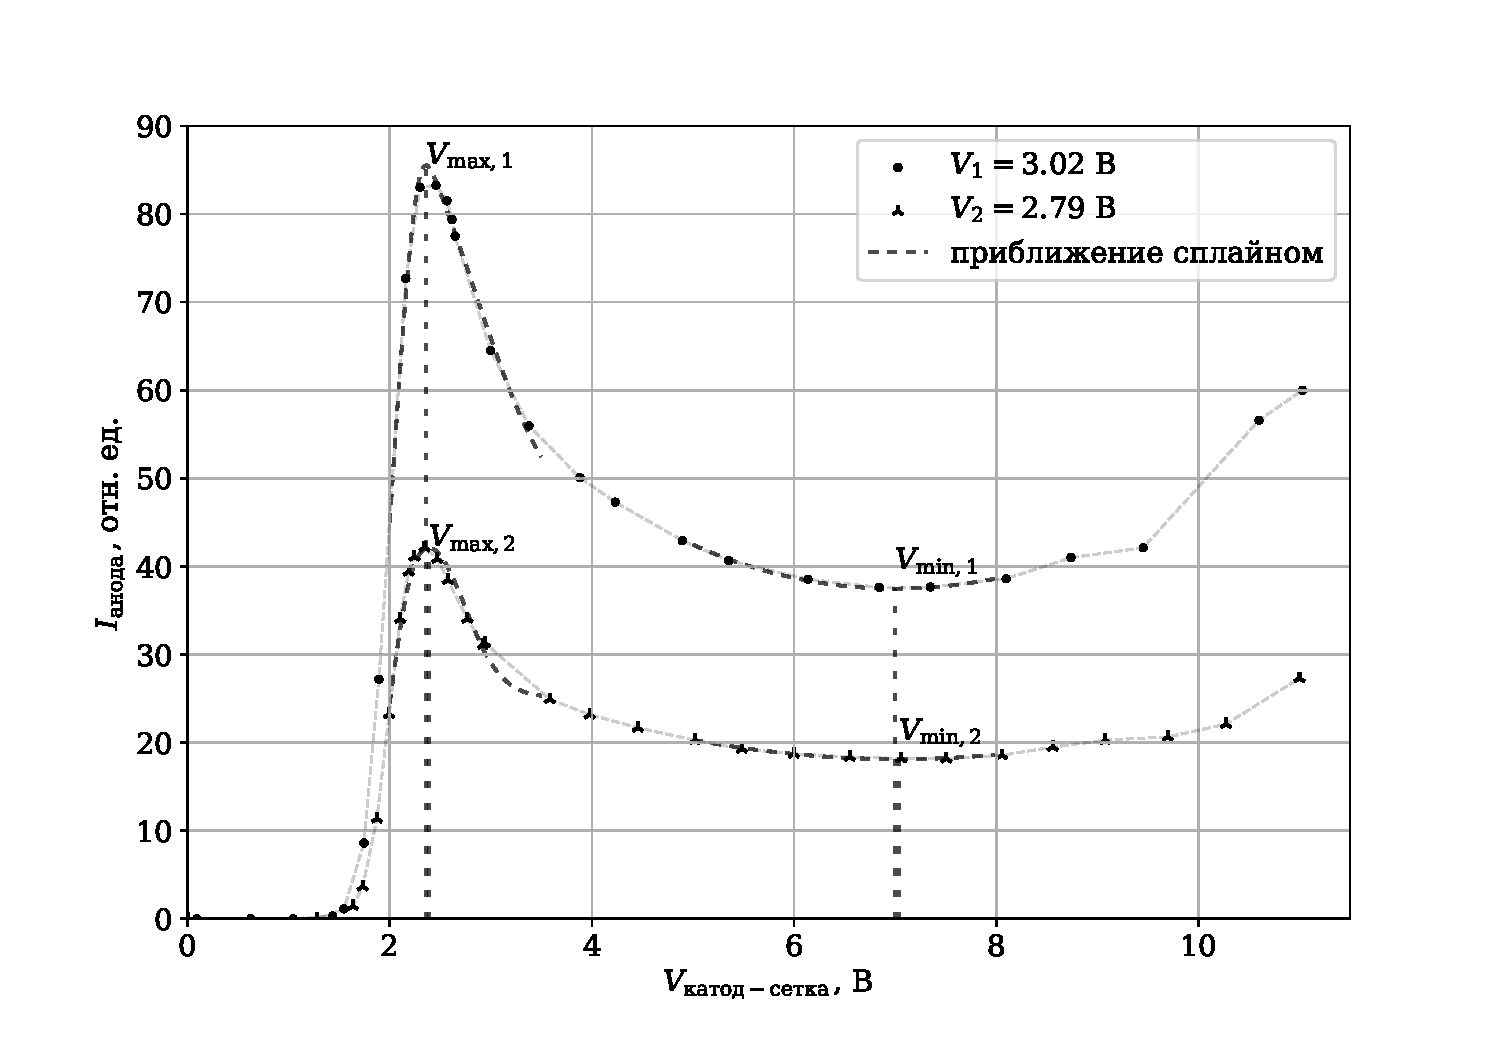
\includegraphics[width=\textwidth]{plot.pdf}
\caption{Графики вольт-амперной характеристики снятые в статическом режиме}
\label{fig:static}
\end{figure}

\begin{figure}
\centering
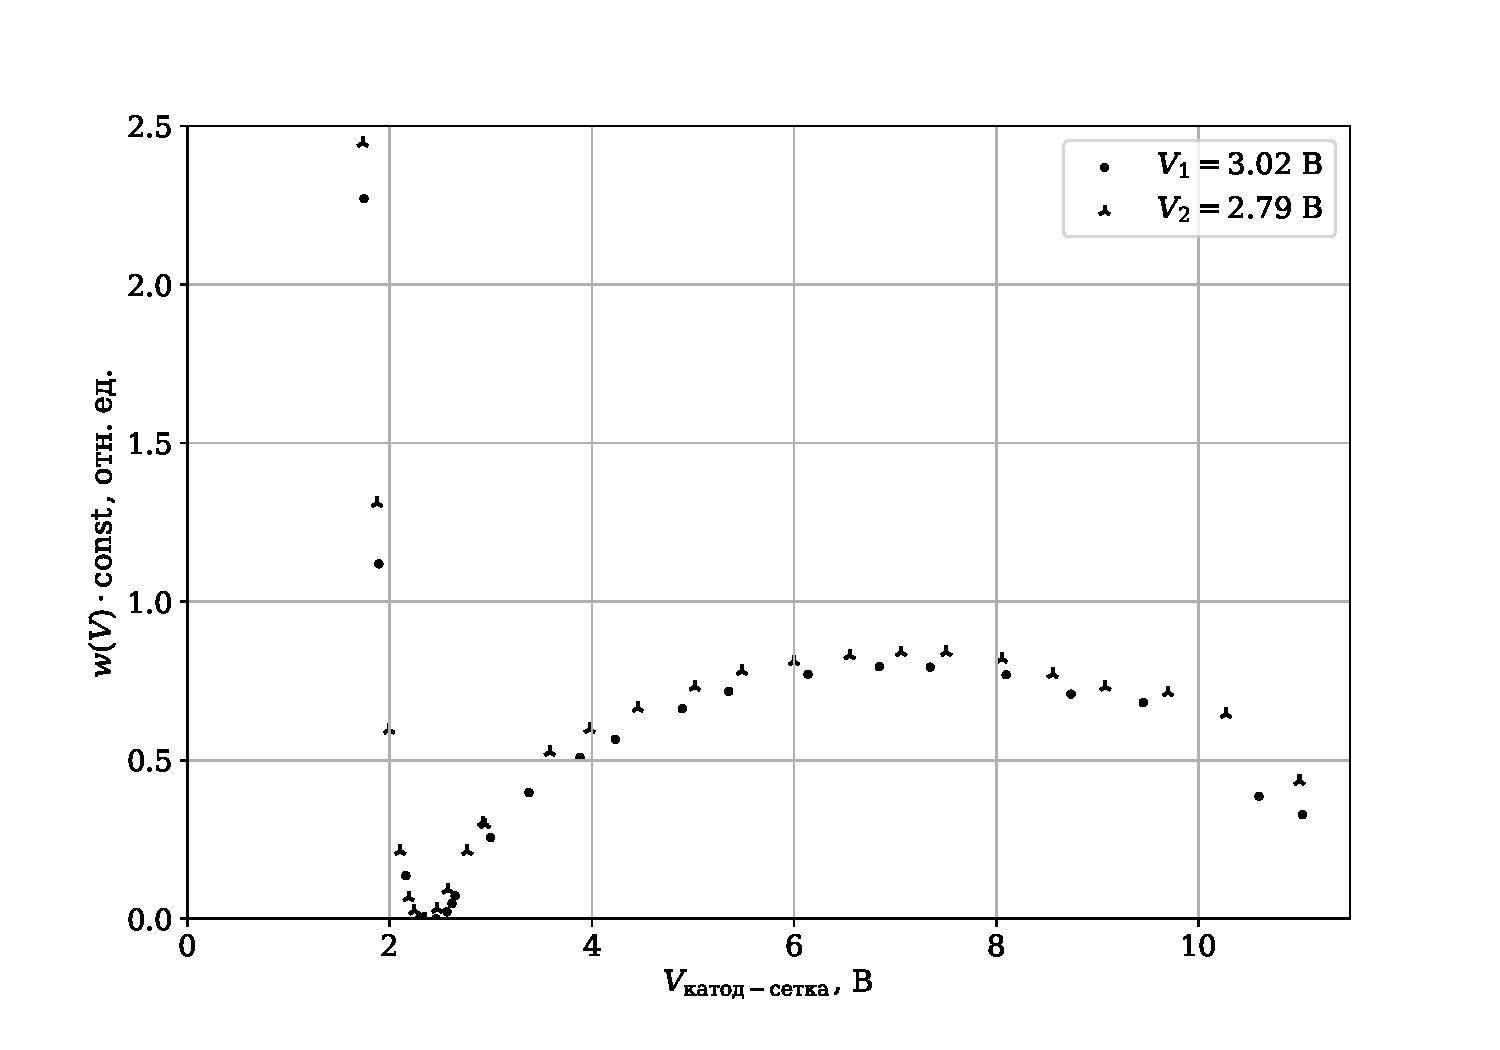
\includegraphics[width=\textwidth]{plot_prob.pdf}
\caption{График вероятности рассеяния электрона}
\label{fig:static_prob}
\end{figure}

\section{Выводы}

\begin{enumerate}
\item Получили качественное изображение вольт-амперной характеристики тиратрона динамическим способом - при помощи источника переменного напряжения и электронного осциллографа. Эта характеристика неточной из-за значительного искажения изображения.
\item Основывая на полученной динамическим способом вольт-амперной характеристики напряжение максимума и минимума пропускания, а также напряжение пробоя.
\item По напряжению максимума и минимума оценили размер внешней оболочки ксенона, получили значения в районе $2.7\div4.1$ Å. По данным справочника ковалентный радиус ксенона $r = 130\div140$ Å, что при умножении на два даёт близкое значение к полученным.
\item Попытались оценить глубину потенциальной ямы атома, что не удалось из-за высокой погрешности.
\item Статическим способом сняли более точную вольт-амперную характеристику.
\item По новой ВАХ нашли размер внешней оболочки ксенона $l = 3.18 \pm 0.07$ Å и глубину потенциальной ямы атома $U_0 = 1.7 \pm 0.1$ В.
\item Построили график зависимости вероятности рассеяния электрона от напряжения.
\end{enumerate}


\medskip\hrule\medskip

\end{document}
